% Diagrama en bloques del CI, explicación de cada una de las partes, 
% explicación de por que no es un chip completo y cuál fue la idea esta 
% implementación, funcionamiento teórico, detalles de la implementación 
% relacionados al proceso CMOS (Puente de diodos)
\chapter{Diseño del transponder de RFID}

En este capítulo se verán los objetivos del diseño del dispositivo, 
cuales son sus alcances y se mencionarán los puntos clave a la hora de 
obtener un dispositivo funcional. Luego se verá un panorama general 
del funcionamiento a través de un diagrama en bloques y se finalizará 
el capítulo dando detalles acerca de la implementación, como por 
ejemplo el proceso de fabricación y sus características principales.


\section{Objetivos del diseño}

En este trabajo el diseño del circuito integrado está orientado a obtener un 
prototipo de un \emph{tag} de RFID tratando de dejar de lado los detalles 
que no hacen a la implementación del protocolo y teniendo en mente la 
posibilidad de ampliar su funcionalidad a través de un microcontrolador o 
FPGA externo. Por este motivo se decidió implementar solo la parte física 
del protocolo, es decir, la recepción, transmisión y reconocimiento de la 
información, así como también la obtención de la energía; dejando la 
implementación de la lógica del protocolo ---el algoritmo anti-colisión, el 
armado de paquetes, etc.--- para trabajos posteriores. El bloque diseñado
puede ser en futuros diseños usado como bloque de propiedad intelectual (IP)
formando parte de un \emph{tag} completo.

Por el lado de la transmisión y recepción de información se le dio mayor 
importancia al reconocimiento de los bits y las tramas y a la codificación y 
envío de los datos, ya que éstas son las unidades básicas descriptas en las 
partes dos y tres de la norma, y a partir de ellas puede construirse toda la 
lógica del protocolo anti-colisión y los paquetes de nivel superior de la 
cuarta parte del estándar.

Por el lado de la energía el objetivo principal del diseño es lograr 
alimentar los circuitos digitales con la señal de RF captada por la antena y 
en lo posible no utilizar elementos externos (como por ej. capacitores para 
el filtrado y mantenimiento de la tensión de alimentación). El mayor desafío 
en este sentido es mantener a los circuitos digitales alimentados mientras 
se recibe información del lector, ya que en esos momentos se producen las 
pausas en la señal de RF y por lo tanto no se recibe energía.

Durante el diseño no se tendrán en cuenta las posibles variaciones de 
temperatura, ya que lo que se trata de obtener es un prototipo para realizar 
pruebas de laboratorio y no para desempeñarse en un ambiente productivo. 
Tampoco se tendrán en cuenta los parámetros estadísticos del proceso 
---además de no contar con ellos--- pero sí se realizarán simulaciones con 
los modelos de los extremos estadísticos (\emph{corner parameters}).

\section{Descripción general del funcionamiento}

En la figura \ref{fig:DiagramaEnBloquesCI} se observa el diagrama en bloques 
del circuito integrado. La señal de RF es recibida por la antena, que forma 
el bloque llamado <<Interfaz Inductiva>>, e ingresa directamente al chip, 
sirviendo de señal de entrada para varios bloques. 

El bloque <<Regulador/Limitador de tensión>> es el encargado de mantener la 
tensión en la entrada del chip, donde se encuentra conectada la antena, por 
debajo de la tensión máxima del proceso CMOS y de esta forma evitar que se 
deterioren los gates de los transistores conectados a esa entrada. Como se 
verá más adelante, la amplitud de la tensión en la antena depende de varios 
factores, entre ellos el coeficiente de acoplamiento, el consumo del chip y 
la intensidad de campo magnético. Como se mostró en la tabla \ref
{tab:NivelesDeCampo}, la intensidad de campo magnético está acotada por el 
estándar al rango de \SI[per-mode=symbol]{1.5}{\ampere\per\meter} a \SI
[per-mode=symbol]{7.5}{\ampere\per\meter}. El circuito integrado debe 
funcionar sin inconvenientes dentro de este amplio rango de intensidades, lo 
que hace necesario el agregado del bloque regulador de tensión. Como se verá 
en detalle más adelante, este bloque controla la tensión inducida variando 
la carga vista por la antena.

El bloque <<Rectificador + Filtro>> es el encargado de alimentar los 
circuitos digitales y demás bloques analógicos, y lo hace rectificando la 
onda senoidal recibida en la antena y luego filtrándola a través de un 
capacitor de gran capacidad. Este capacitor debe ser tal que conserve la 
carga durante el tiempo de duración de las pausas en la señal de RF, y de 
esta forma evitar que el estado de los circuitos digitales se vea alterado 
durante ese intervalo.

El <<Detector de Pausas>> se encarga de traducir las pausas en la señal de 
RF a los niveles lógicos del bloque digital, para que este último pueda usar 
como entrada de datos. No es más que un detector de envolvente seguido de 
una serie de inversores que se cambian de estado para indicar que se está en 
una pausa.

\begin{figure}
	\centering
	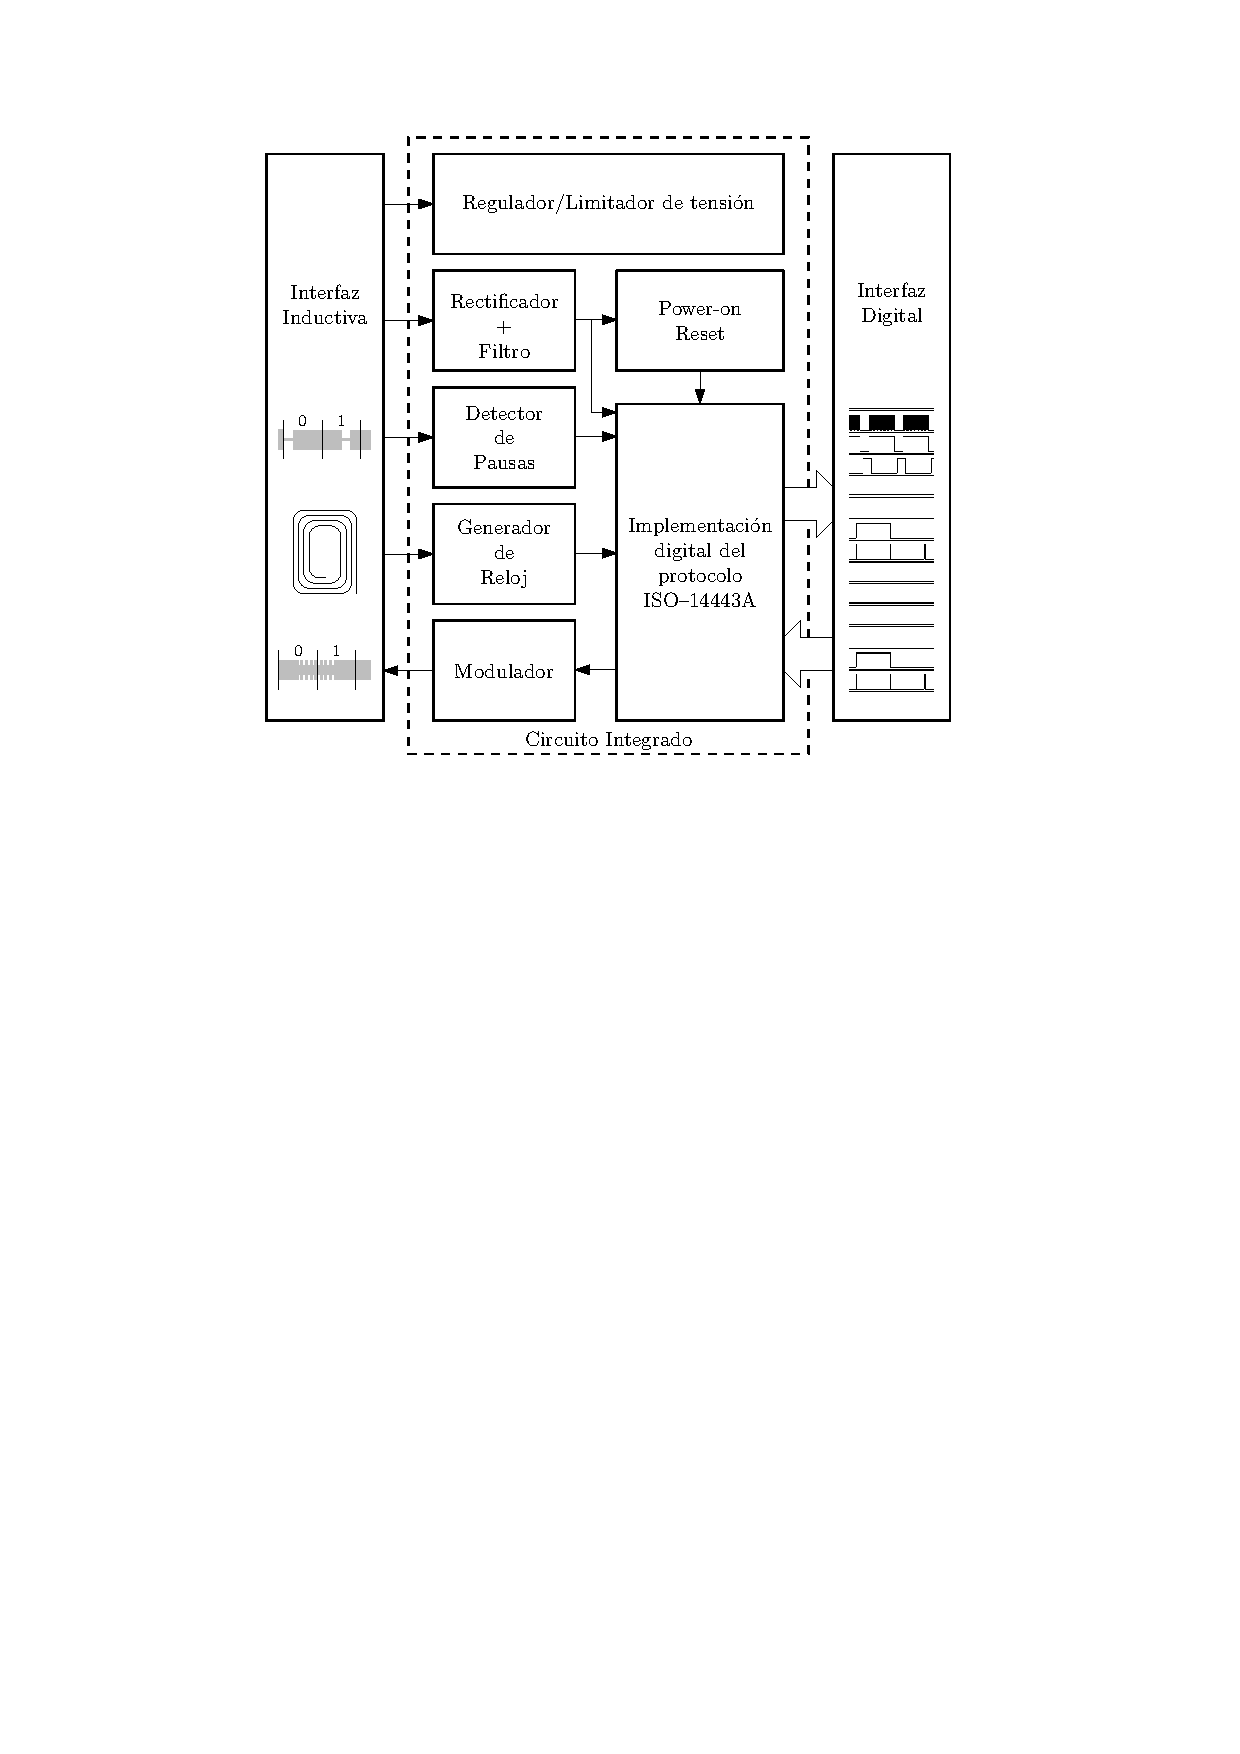
\includegraphics[width=0.8\linewidth]{diagrama_en_bloques}
	\caption{Diagrama en bloques del circuito integrado y sus interfaces.}
	\label{fig:DiagramaEnBloquesCI}
\end{figure}

El bloque <<Generador de Reloj>> recibe la señal de RF y a partir de ella 
produce una señal cuadrada de la misma frecuencia. Luego la señal cuadrada 
será utilizada por los circuitos digitales como reloj. Es muy importante que 
no se produzcan \emph{glitches}, sobre todo al comenzar y finalizar las 
pausas de RF, ya que esto podría desincronizar los registros del bloque 
digital. También es importante desde el punto de vista del consumo que los 
flancos sean de corta duración para reducir la potencia dinámica consumida.

El <<Modulador>> realiza el proceso de modulación de carga para transmitir 
información hacia el lector. Se trata de un modulador capacitivo, ya que 
conecta un par de capacitores directamente a la entrada de la antena, lo que 
incrementa la carga vista por la misma y posibilita el envío de datos. Este 
bloque no realiza la codificación de la información, ni la modulación con 
subportadora, ya que estos procesos fueron resueltos digitalmente.

En el bloque digital se implementa la codificación y decodificación de los 
bits y el reconocimiento y armado de las tramas. La información es recibida 
a través de la modulación de amplitud de la señal de RF y el <<Detector de 
Pausas>> es el encargado de traducir esta modulación a una señal digital de 
unos y ceros lógicos. El bloque digital toma muestras de esta señal y de 
esta forma decodifica los bits recibidos. Ahora bien, como se vio en la 
descripción de la tercera parte del estándar (sección \ref{sec:ISO14443_3}), 
cada trama recibida está compuesta por un bit de <<Inicio>>, dependiendo del 
tipo de trama puede existir uno de paridad, y finalmente un bit de <<Fin>> 
de comunicación. Estas marcas son detectadas por el bloque digital, 
interpretadas y separadas de la información útil, que es presentada por el 
bloque <<Interfaz Digital>> al exterior del circuito integrado. Cabe 
destacar que el sistema digital interpreta cualquier tipo de trama, de 
cualquier largo, siempre y cuando respete la estructura del estándar. 
Además, desde el momento en que se recibe el bit de <<Fin>> de comunicación, 
se dispara un contador que controla el \emph{Frame Delay Time} (FDT) e 
inhibe la transmisión de datos hasta que se cumpla el tiempo dictaminado por 
la norma.

Para la transmisión desde la PICC hacia el PCD el bloque digital cuenta con 
una entrada de datos a través de la <<Interfaz Digital>> que permite 
realizar una carga tipo \emph{shit register} ---es decir, los bits se cargan 
en forma secuencial, de a uno por vez--- y una señal de comando que indica 
el inicio de la transmisión. A través de esta interfaz es posible enviar de 
uno a ocho bits de datos. El bloque digital se encarga de respetar el FDT e 
iniciar la transmisión una vez concluido éste, y por otro lado agrega los 
bits de inicio, paridad y fin de comunicación. Además realiza la modulación 
de los bits con la subportadora descripta en la sección \ref{sec:ISO14443_2}.

Para que el circuito digital comience a trabajar en un estado conocido, el 
bloque <<Power-on Reset>> se encarga de enviar la señal de reset cuando la 
tensión de alimentación alcanza un nivel mínimo que permite el 
funcionamiento del dispositivo. Para ello monitorea la tensión a la salida 
del bloque de rectificación y filtrado y, a través de una comparación de 
parámetros de transistores, mantiene la señal de reset en alto hasta que se 
cumple la condición de funcionamiento.

Por último, el bloque <<Interfaz Digital>> físicamente no es más que una 
serie de buffers digitales con el propósito de manejar adecuadamente las 
mayores capacidades del exterior del circuito integrado. Lo interesante de 
esta interfaz es que las señales involucradas en la recepción y transmisión 
de datos fueron pensadas de forma tal que pudieran conectarse entre sí. 
Cuando se hace esto, al recibir una trama de un byte éste se carga 
directamente en el registro de transmisión y es devuelto al lector en cuanto 
se cumple el FDT. De esta forma puede utilizarse el circuito integrado de 
forma autónoma como un tag RFID que realiza un eco de un byte.

\section{Implementación}

El circuito integrado fue fabricado a través de MOSIS \cite{MosisWeb} en 
el proceso de C5N de la empresa \emph{ON Semiconductor}. Se trata de 
un proceso de fabricación CMOS estándar de \SI{0.5}{\micro\meter} de 
longitud de canal. El proceso cuenta con tres capas de metal con la 
posibilidad de superponer contactos y dos capas de polisilicio con las 
que pueden fabricarse capacitores PiP (\emph{poly2 sobre poly}) de 
\SI[per-mode=symbol]{950}{\atto\farad\per\micro\meter\squared} y 
además cuenta con una máscara especial para incrementar la 
resistencia de la segunda capa de polisilicio, con la que pueden 
fabricarse resistores de alto valor. La tensión nominal de trabajo de 
es \SI{5}{\volt} y el área disponible para el diseño fue de 
\(\SI{1500}{\micro\meter}\times\SI{750}{\micro\meter}\).

El diseño analógico del transponder se realizó primero utilizando el 
programa para simulación de circuitos \emph{LTSpice} \cite{LTSpice}, 
de \emph{Linear Technology}, utilizando para ello los modelos de SPICE 
de los dispositivos brindados por MOSIS. Estos modelos son de tipo 
BSIM3, en su versión 3.1, y son creados a partir de  
mediciones realizadas sobre los dispositivos una vez que estos han 
sido fabricados. Algunos datos interesantes del proceso pueden verse 
en las tablas \ref{tab:DatosProcesoTransistores}, 
\ref{tab:DatosProcesoResistencias} y 
\ref{tab:DatosProcesoCapacidades}. Los datos allí volcados 
corresponden a las mediciones realizadas sobre \emph{wafers} fabricados 
en la corrida V33R, la anterior a la que finalmente se usó para 
fabricar el chip. Por lo tanto puede suponerse que los valores allí 
mostrados serán los típicos obtenidos en el circuito integrado, pero 
también deben esperarse variaciones de hasta un 20\% en los parámetros 
más sensibles.

\begin{table}
	\centering
	\begin{tabu}{lcrrc}
		\toprule
		Parámetro & W/L & Canal N & Canal P & Unidad \\
		\midrule
		\textbf{Mínimo}     & \SI{3.0}{}/\SI{0.6} &           &            & \si{\micro\meter} \\
		\(V_{th}\) &                     & \SI{0.80} & \SI{-0.94} & \si{\volt} \\
		\midrule
		\textbf{Corto}     & \SI{20.0}{}/\SI{0.6} &           &            & \si{\micro\meter} \\
		\(V_{th}\) &                     & \SI{0.69} & \SI{-0.92} & \si{\volt} \\
		\midrule
		\textbf{Largo}     & \SI{50.0}{}/\SI{50.0} &           &            & \si{\micro\meter} \\
		\(V_{th}\) &                     & \SI{0.71} & \SI{-0.97} & \si{\volt} \\
		\midrule
		\(k'\,\left(\sfrac{\mu_{0} C_{ox}}{2}\right)\) & & \SI{57.4}{} & \SI{-18.7}{} & \si[per-mode=symbol]{\micro\ampere\per\volt\squared} \\
		\bottomrule
	\end{tabu}
	\caption{Parámetros de los transistores típicos en la corrida V33R. El 
	circuito integrado fue fabricado en la corrida siguiente.}
	\label{tab:DatosProcesoTransistores}
\end{table}

\begin{table}
	\centering
	\begin{tabu}{lcccccccccc}
		\toprule
		Resistencia & N+ & P+ & poly & poly2 (HR) & poly2 & Unidad\\
		\midrule
		Capa & \SI{81.7} & \SI{105.1} & \SI{23.0} & \SI{1030} & \SI{41.2} & \(\sfrac{\si{\ohm}}{\square}\) \\
		Contacto & \SI{58.7} & \SI{144.5} & \SI{15.0} &  ~    & \SI{24.8} & \si{\ohm} \\
		\bottomrule
		\addlinespace
		\toprule
		Resistencia & ~ & M1 & M2 & M3 & Nwell & Unidad \\
		\midrule
		Capa & ~ & \SI{0.09} & \SI{0.09} & \SI{0.05} & \SI{824} & \(\sfrac{\si{\ohm}}{\square}\) \\
		Contacto & ~ & ~ & \SI{0.86} & \SI{0.9} & ~ & \si{\ohm} \\
		\bottomrule
	\end{tabu}
	\caption{Resistencias típicas de las capas y los contactos en la 
	corrida V33R.}
	\label{tab:DatosProcesoResistencias}
\end{table}

\begin{table}
	\centering
	\resizebox{\textwidth}{!}{
		\small
		\begin{tabu}{lccccccccc}
			\toprule
			Capacidad & N+ & P+ & poly & poly2 & M1 & M2 & M3 & Nwell & Unidad \\
			\midrule
			Área (substrate)  &    425& 734&   87 &   ~  &   28 & 12 &  7  &  38 & \si[per-mode=symbol]{\atto\farad\per\micro\meter\squared} \\
			Área (N+active)   &   ~   &  ~ & \textbf{2474} & ~  & \textbf{36} & 16 & 11  &  ~  & \si[per-mode=symbol]{\atto\farad\per\micro\meter\squared} \\
			Área (P+active)   &   ~   &  ~ & 2393 &   ~  &   ~  & ~  &  ~  &  ~  & \si[per-mode=symbol]{\atto\farad\per\micro\meter\squared} \\
			Área (poly)       &   ~   &  ~ &  ~   &  \textbf{885} &   65 & 15 &  9  &  ~  & \si[per-mode=symbol]{\atto\farad\per\micro\meter\squared} \\
			Área (poly2)      &   ~   &  ~ &  ~   &   ~  &   57 & ~  &  ~  &  ~  & \si[per-mode=symbol]{\atto\farad\per\micro\meter\squared} \\
			Área (metal1)     &   ~   &  ~ &  ~   &   ~  &   ~  & 29 & 12  &  ~  & \si[per-mode=symbol]{\atto\farad\per\micro\meter\squared} \\
			Área (metal2)     &   ~   &  ~ &  ~   &   ~  &   ~  & ~  & 29  &  ~  & \si[per-mode=symbol]{\atto\farad\per\micro\meter\squared} \\
			Borde (substrate) &    336& 234&  ~   &   ~  &   53 & 34 & 23  &  ~  & \si[per-mode=symbol]{\atto\farad\per\micro\meter} \\
			Borde (poly)      &   ~   & ~  &  ~   &   ~  &   67 & 38 & 28  &  ~  & \si[per-mode=symbol]{\atto\farad\per\micro\meter} \\
			Borde (metal1)    &   ~   & ~  &  ~   &   ~  &   ~  & 47 & 32  &  ~  & \si[per-mode=symbol]{\atto\farad\per\micro\meter} \\
			Borde (metal2)    &   ~   & ~  &  ~   &   ~  &   ~  & ~  & 46  &  ~  & \si[per-mode=symbol]{\atto\farad\per\micro\meter} \\
			\bottomrule
		\end{tabu}
	}
	\caption{Capacidades típicas entre capas y/o junturas en la corrida 
	V33R. Los valores usados en el diseño fueron resaltados.}
	\label{tab:DatosProcesoCapacidades}
\end{table}

El diseño digital fue codificado utilizando el lenguaje descriptor de 
hardware \emph{Verilog} \cite{Verilog} y en principio se utilizaron 
herramientas libres, como \emph{Icarus Verilog} \cite{IVerilog} y 
\emph{GTKwave} \cite{GTKWave} para realizar la verificación 
funcional de cada uno de los bloques y luego de todo el conjunto. Una 
vez verificado su funcionamiento el diseño fue procesado con las 
herramientas de \emph{Synopsys Inc.}, \emph{DC Compiler} 
\cite{SynopsysDC} y \emph{IC Compiler} \cite{SynopsysICCompiler}. Con 
el primero se realizó la síntesis del RTL para obtener una 
\emph{netlist} de compuertas digitales. Para ello se utilizó también la 
biblioteca de celdas estándar de la \emph{Oklahoma State University} 
(OSU) \cite{OSUstandardCells}, que cuenta con un conjunto de 
compuertas digitales caracterizadas para el proceso C5N. El 
posicionado y conexionado (\emph{place\&route}) de las celdas fue 
realizado con la segunda herramienta, \emph{IC Compiler}, con la que 
se obtuvo el trazado físico (\emph{layout}) final de la parte digital 
del transponder. El \emph{layout} fue exportado en formato GDSII para 
luego ser agregado al diseño final.

Finalmente, los circuitos analógicos y el bloque digital fueron 
trasladados a la herramienta de \emph{Mentor Graphics} 
\cite{MentorCustomIC} con la que se realizaron las simulaciones y el 
\emph{layout} final de todo el chip. Junto con la herramienta se 
utilizó el kit de diseño del proceso C5N cedido por MOSIS, donde 
se define el set de máscaras a utilizar para el trazado del 
\emph{layout} y que contiene las reglas del proceso con los tamaños y 
distancias mínimas entre máscaras. Además contiene una serie de 
dispositivos predefinidos como transistores, resistores y capacitores. 
El esquemático está vinculado con el \emph{layout} de forma tal que 
cada uno de esos dispositivos se coloca en el \emph{layout} según los 
tamaños definidos en el esquemático. A esta forma de trabajo se la 
llama \emph{Schematic Driven Layout} (SDL) y fue la que se utilizó 
para el trazado de los dispositivos y el conexionado de los diferentes 
bloques.
